% UiS Beamer presentation (http://ctan.org/pkg/beamer)
% Modified by Nithiya Streethran (nmstreethran@gmail.com) using uisbeamer.sty
% Licence: GNU General Public License v3 (https://www.gnu.org/licenses/gpl-3.0.en.html)
% University of Stavanger (UiS) (https://www.uis.no/)

% DOCUMENT CONFIGURATION AND PROPERTIES -------------------------------
\documentclass[aspectratio=169]{beamer} % aspect ratio for widescreen
\mode<presentation> {}

% define shortcuts to document properties https://en.wikibooks.org/wiki/TeX/def
\def \auth {Author} % author
\def \prestitle {The presentation title, which can be long ...} % presentation title; maximum three lines in the title slide
\def \titlesize {\LARGE} % title font size; maximum four lines at \LARGE; if you would like to change the font size, use one of these other font size commands: https://www.overleaf.com/learn/latex/Font_sizes,_families,_and_styles#Reference_guide 
\def \subt {Subtitle} % subtitle/event name; leave empty {} if none
\renewcommand \date {\today} % date
\def \email {emailid@mail.com} % email
\def \ending {Thank you for your attention!} % ending for end frame
\def \licenseurl {https://www.gnu.org/licenses/gpl-3.0.en.html} % license URL; leave empty {} if none
\def \copyright {Copyright \textcopyright~\the\year{}~by \author. Licensed under the GNU General Public License v3.} % copyright info; leave empty {} if none
\def \subject {Subject} % subject of the presentation; leave empty {} if none
\def \keywords {keyword1, keyword2} % keywords; leave empty {} if none

% import UiS beamer style file
\usepackage{uisbeamer}

% import bibliography file
\addbibresource{sample.bib} % sample bibliography

%%%%%%%%%%%%%%%%%%%%%%%%%%%
\begin{document}

% TITLE SLIDE -------------------------------
\begingroup
\titlebg % set title frame background; do this before beginning the frame
\begin{frame}[t]
	\maketitle
\end{frame}
\endgroup

% MAIN BODY SLIDES ----------------------------------
\bodybg % set main body frames' background 
\begin{frame}{Table of Contents} % Table of contents slide, comment this block out to remove it
\tableofcontents % Throughout your presentation, if you choose to use \section{} and \subsection{} commands, these will automatically be printed on this slide as an overview of your presentation
\end{frame}

%------------------------------------------------
\section{First Section} % Sections can be created in order to organize your presentation into discrete blocks, all sections and subsections are automatically printed in the table of contents as an overview of the talk
%------------------------------------------------

\subsection{Subsection Example} % A subsection can be created just before a set of slides with a common theme to further break down your presentation into chunks

\begin{frame}{Table of Contents} 
\tableofcontents[currentsection] 
\end{frame}

\begin{frame}{Paragraphs of Text}
Sed iaculis dapibus gravida. Morbi sed tortor erat, nec interdum arcu. Sed id lorem lectus. Quisque viverra augue id sem ornare non aliquam nibh tristique. Aenean in ligula nisl. Nulla sed tellus ipsum. Donec vestibulum ligula non lorem vulputate fermentum accumsan neque mollis.\\~\\

Sed diam enim, sagittis nec condimentum sit amet, ullamcorper sit amet libero. Aliquam vel dui orci, a porta odio. Nullam id suscipit ipsum. Aenean lobortis commodo sem, ut commodo leo gravida vitae. Pellentesque vehicula ante iaculis arcu pretium rutrum eget sit amet purus. Integer ornare nulla quis neque ultrices lobortis. Vestibulum ultrices tincidunt libero, quis commodo erat ullamcorper id.
\end{frame}

%------------------------------------------------

\begin{frame}{Bullet Points}
\begin{itemize}
\item Lorem ipsum dolor sit amet, consectetur adipiscing elit
\item Aliquam blandit faucibus nisi, sit amet dapibus enim tempus eu
\item Nulla commodo, erat quis gravida posuere, elit lacus lobortis est, quis porttitor odio mauris at libero
\item Nam cursus est eget velit posuere pellentesque
\item Vestibulum faucibus velit a augue condimentum quis convallis nulla gravida
\end{itemize}
\end{frame}

%------------------------------------------------

\begin{frame}{Blocks of Highlighted Text}
\begin{block}{Block 1}
Lorem ipsum dolor sit amet, consectetur adipiscing elit. Integer lectus nisl, ultricies in feugiat rutrum, porttitor sit amet augue. Aliquam ut tortor mauris. Sed volutpat ante purus, quis accumsan dolor.
\end{block}

\begin{block}{Block 2}
Pellentesque sed tellus purus. Class aptent taciti sociosqu ad litora torquent per conubia nostra, per inceptos himenaeos. Vestibulum quis magna at risus dictum tempor eu vitae velit.
\end{block}

\begin{block}{Block 3}
Suspendisse tincidunt sagittis gravida. Curabitur condimentum, enim sed venenatis rutrum, ipsum neque consectetur orci, sed blandit justo nisi ac lacus.
\end{block}
\end{frame}

%------------------------------------------------

\begin{frame}{Multiple Columns}
\begin{columns}[c] % The "c" option specifies centered vertical alignment while the "t" option is used for top vertical alignment

\column{.45\textwidth} % Left column and width
\textbf{Heading}
\begin{enumerate}
\item Statement
\item Explanation
\item Example
\end{enumerate}

\column{.5\textwidth} % Right column and width
Lorem ipsum dolor sit amet, consectetur adipiscing elit. Integer lectus nisl, ultricies in feugiat rutrum, porttitor sit amet augue. Aliquam ut tortor mauris. Sed volutpat ante purus, quis accumsan dolor.

\end{columns}
\end{frame}

%------------------------------------------------
\section{Second Section}

\begin{frame}{Table of Contents} 
\tableofcontents[currentsection] 
\end{frame}
%------------------------------------------------

\begin{frame}{Table}
\begin{table}
\setbeamertemplate{caption}{\insertcaption} % if label is not required
\caption{Table caption}
\begin{tabular}{l l l}
\toprule
\textbf{Treatments} & \textbf{Response 1} & \textbf{Response 2}\\
\midrule
Treatment 1 & 0.0003262 & 0.562 \\
Treatment 2 & 0.0015681 & 0.910 \\
Treatment 3 & 0.0009271 & 0.296 \\
\bottomrule
\end{tabular}
\end{table}
\end{frame}

%------------------------------------------------

\begin{frame}{Theorem}
\begin{theorem}[Mass--energy equivalence]
$E = mc^2$
\end{theorem}
\end{frame}

%------------------------------------------------

\begin{frame}[fragile]{Verbatim} % Need to use the fragile option when verbatim is used in the slide
\begin{example}[Theorem Slide Code]
\begin{verbatim}
\begin{frame}
\frametitle{Theorem}
\begin{theorem}[Mass--energy equivalence]
$E = mc^2$
\end{theorem}
\end{frame}\end{verbatim}
\end{example}
\end{frame}

%------------------------------------------------

\begin{frame}{Figure}
Uncomment the code on this slide to include your own image from the same directory as the template .TeX file.
\begin{figure}
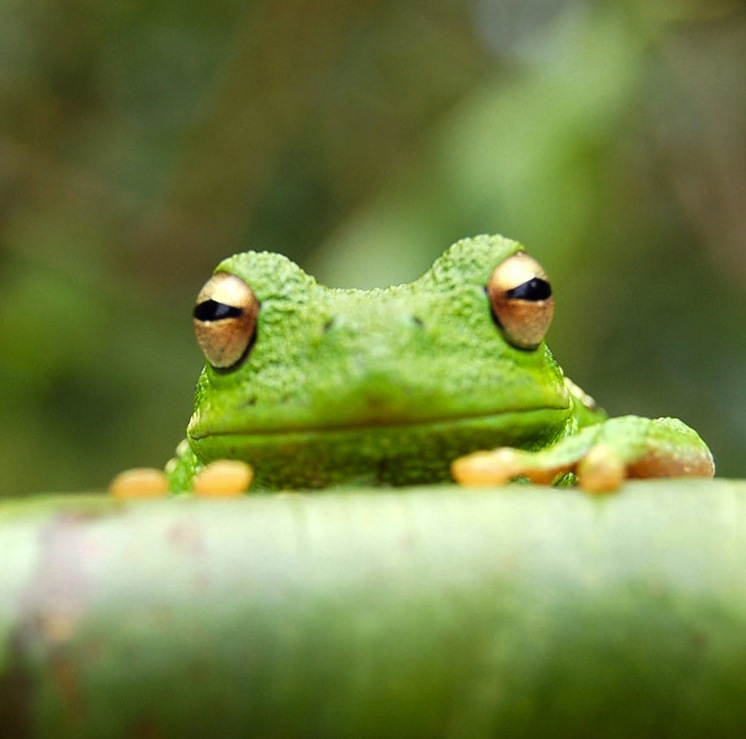
\includegraphics[width=.2\linewidth]{frog}
\setbeamertemplate{caption}{\insertcaption} % if label is not required
\caption{Figure caption}
\end{figure}
\end{frame}

%------------------------------------------------

\begin{frame}[fragile]{Citation} % Need to use the fragile option when verbatim is used in the slide
An example of the \verb|\cite| command to cite within the presentation:\\~

This statement requires a citation \cite{westfahl:space}. This statement requires three citations \cite{angenendt,knuth:ct:b,aristotle:rhetoric}. This statement requires multiple citations \cite{angenendt,knuth:ct:b,aristotle:rhetoric,westfahl:space}.
\end{frame}

% END SLIDE ------------------------------------------------
\begingroup
\titlebg % set frame background (same as title frame)
\begin{frame}[t]
	\makeendframe
\end{frame}
\endgroup

% BACKUP SLIDES -----------------------------------------------
\appendix 
\backupbg % set backup frames' background
\begin{frame}[noframenumbering,plain,allowframebreaks]{References} 
% if you would like a citation which is not used in the main body to be displayed in the references, use the \nocite{bibid} command
\nocite{vangennep:related,ctan}
\printbibliography
\end{frame} % references and backup slides

\end{document}